\paragraph*{Слежение за заданной траекторией}\\
Многозвенный манипулятор представляет из себя систему состоящую из \textit{n} сочленений. Каждое сочленение манипулятора испытывает момент нагрузки, обусловленный гравитационными силами, действующий на последующие сочленения и моменты сил вырабатываемые другими сочленениями, то есть каждое звено влияет на точность перемещения системы по заданной траектории. Следовательно слежение за траекторией можно разделить на две основных задачи. Во-первых, обеспечение слежения за траекторией путем регулирования напряжений в зависимости от информации полученной с датчиков. Во-вторых, компенсация создаваемых моментов сил и нагрузки.\\

В случае одномерного управления момент нагрузки рассматривается как внешний момент $M_l$.
Во второй лабораторной работе вы уже вывели передаточную функция от входа $M_u(s)$ к выходу $ \Theta(s)$ принимая $M_l(s)=0$:\\
\begin{equation}\label{eq:model}
frac{\Theta(s)}{M_u(s)}\approx \frac{1}{s(J_ms+K)},
\end{equation}
где $M_u(s) = \frac{K_m}{R}U(s)$, $K=K_f + \frac{K_eK_m}{R}$. Теперь получим передаточную функцию от входа $M_l(s)$ к выходу $ \Theta(s)$ принимая $U(s)=0$:\\
\begin{equation}\label{eq:model}
frac{\Theta(s)}{M_l(s)}\approx -\frac{1}{s(J_ms+K)},
\end{equation}

Комбинируя передаточные функции (1) и (2) получаем:\\
\begin{equation}\label{eq:model}
\Theta(s) = \frac{1}{s(J_ms + K)}(M_u(s)-M_l(s)) = P(s)(M_u(s) - M_l(s)),
\end{equation}

где \textit{P(s)} передаточная функция математической модели вращательного сочленения с учетом внешних моментов.\\

Первую задачу слежения за траекторией помогает решить ПИД-регулятор. Вы уже знакомы с ПИД-регулятором по скорости изображенном на рис. 4.1\\
\begin{center}
    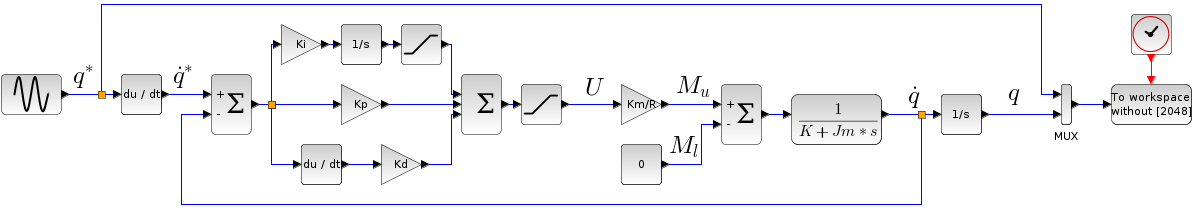
\includegraphics[width=\textwidth]{Lab4/images/Scheme_without.png}\\
    \centering{Рис 4.1 Система моделирования замкнутой системы с ПИД-регулятором}
\end{center}
\vspace{1cm}
 Как видно из ошибки моделирования слежения за траекторией представленной синусом, данной системе не хватает точности позиционирования, то есть манипулятор не точно отрабатывает траекторию.\\
 \vspace{1cm}
 \begin{center}
    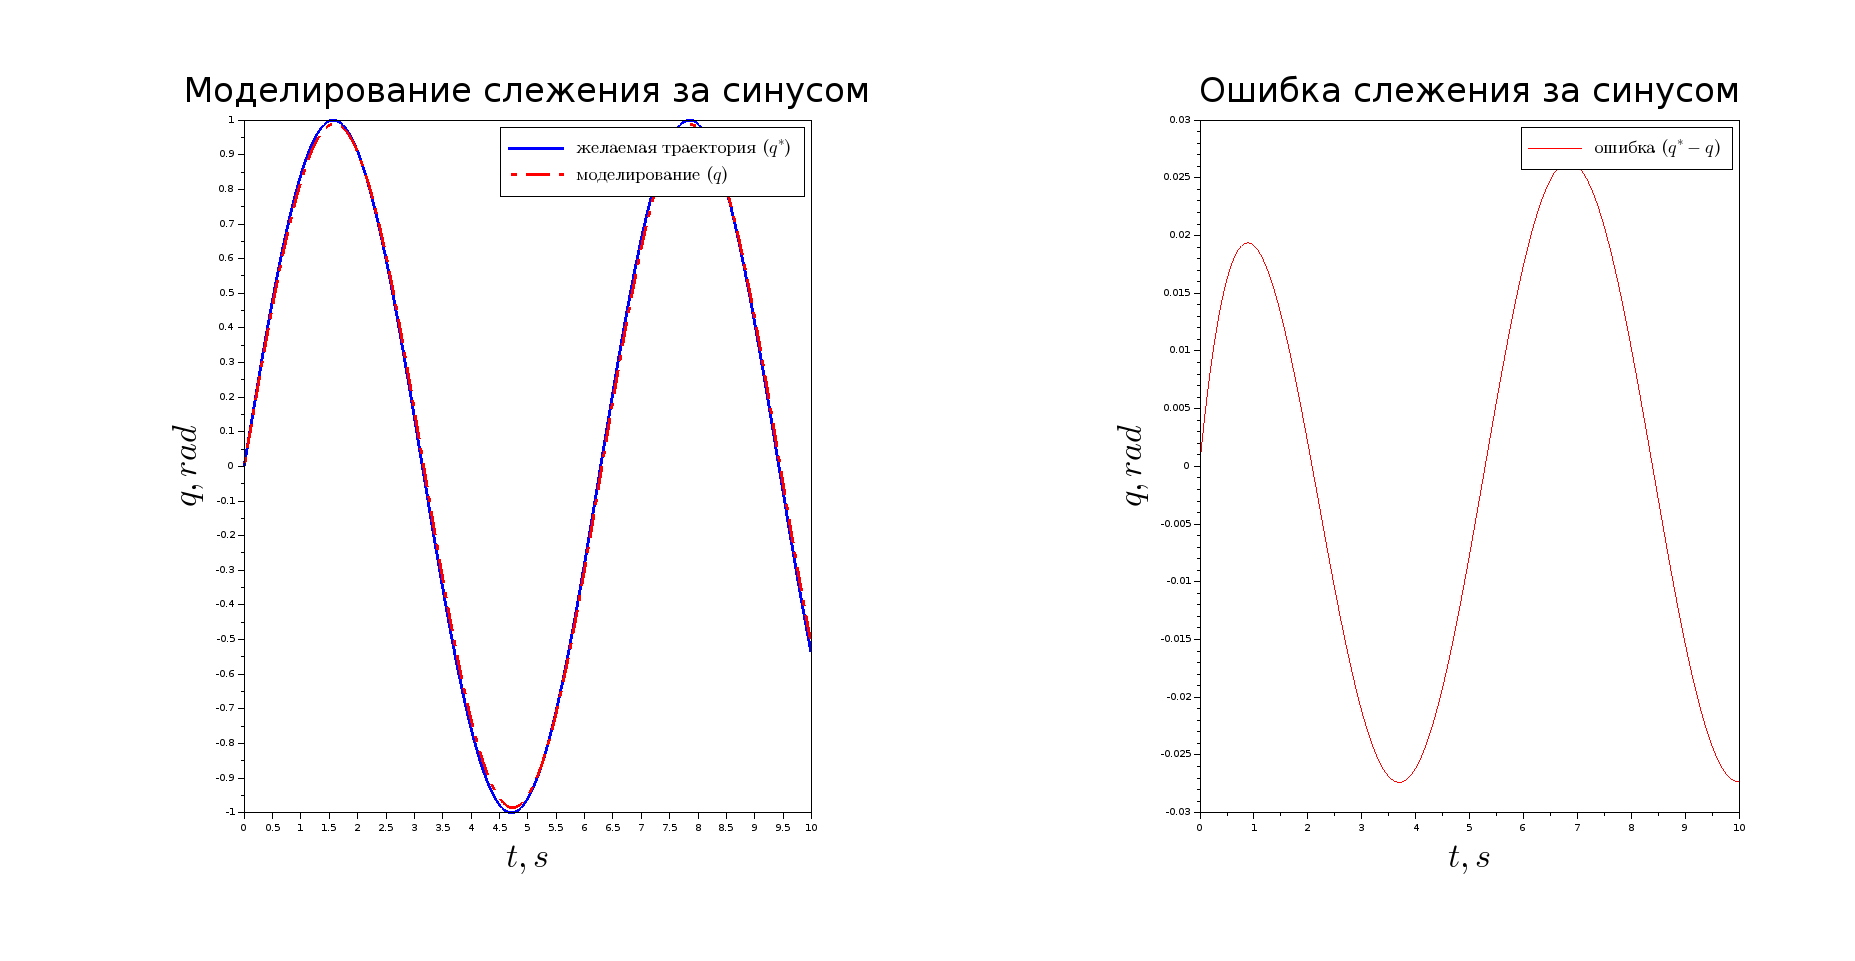
\includegraphics[width=0.8\textwidth]{Lab4/images/Pict_without.png}\\
    \centering{Рис 4.2 Моделирование слежения за синусом одного привода без внешнего воздействия}
\end{center}

\begin{center}
    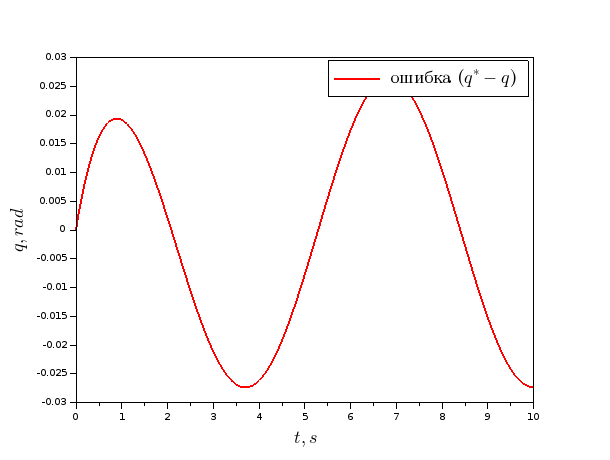
\includegraphics[width=0.8\textwidth]{Lab4/images/Error_without.png}\\
    \centering{Рис 4.3 Ошибка слежения за синусом одного привода без внешнего воздействия}
\end{center}
\vspace{1cm}
Для решения второй задачи слежения за траекторией необходимо сделать траекторный регулятор.Пропорционального регулятора по углу будет вполне достаточно. Реализацию данного регулятора можно найти в схеме моделирования представленной на рис. 4.4. \\
\vspace{1cm}
\begin{center}
    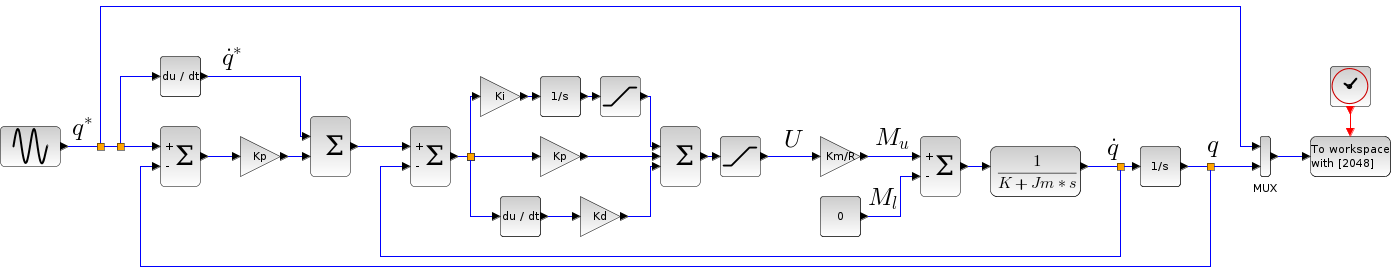
\includegraphics[width=\textwidth]{Lab4/images/Scheme_with.png}\\
    \centering{Рис 4.4 Система моделирования замкнутой системы с траекторным регулятором}
\end{center}
\begin{center}
Как можно заметить после внедрения траекторного регулятора сочленение стало лучше следовать за синусом и порядок ошибки уменьшился.
    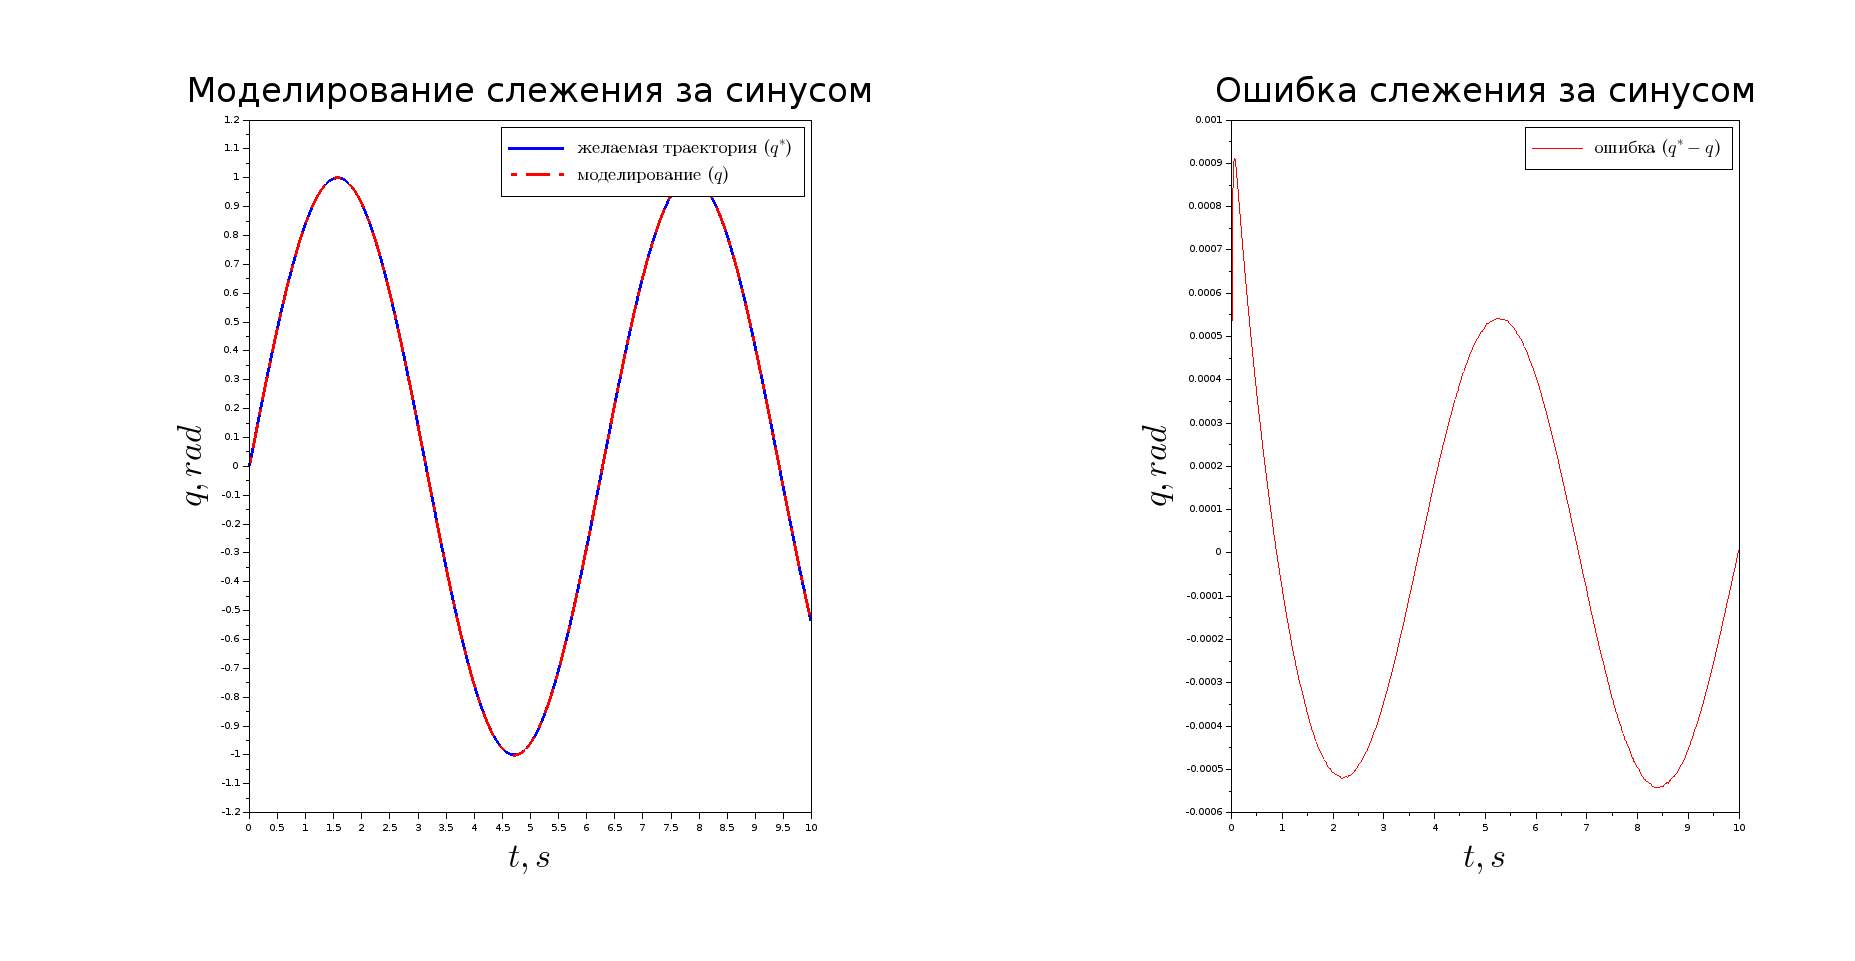
\includegraphics[width=0.8\textwidth]{Lab4/images/Pict_with.png}\\
    \centering{Рис 4.5 Моделирование слежения за синусом одного привода с траекторным регулятором}
\end{center}

\begin{center}
    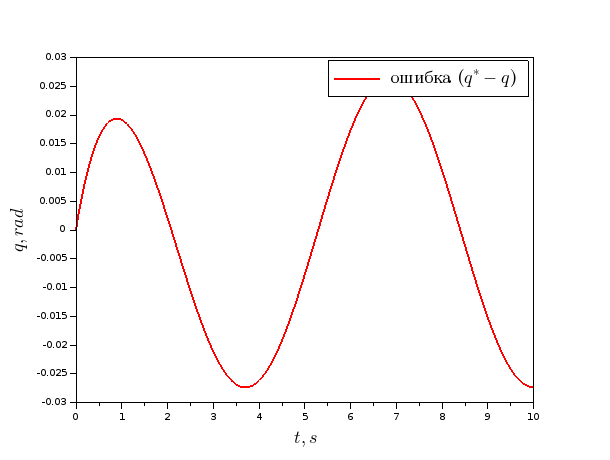
\includegraphics[width=0.8\textwidth]{Lab4/images/Error_without.png}\\
    \centering{Рис 4.6 Ошибка слежения за синусом одного привода с траекторным}
\end{center}
\newpage
Чтобы наглядно показать влияние траекторного регулятора на точность следования желаемой траектории на рисунке 4.7 приведен график сравнения двух ошибок.
\begin{center}
    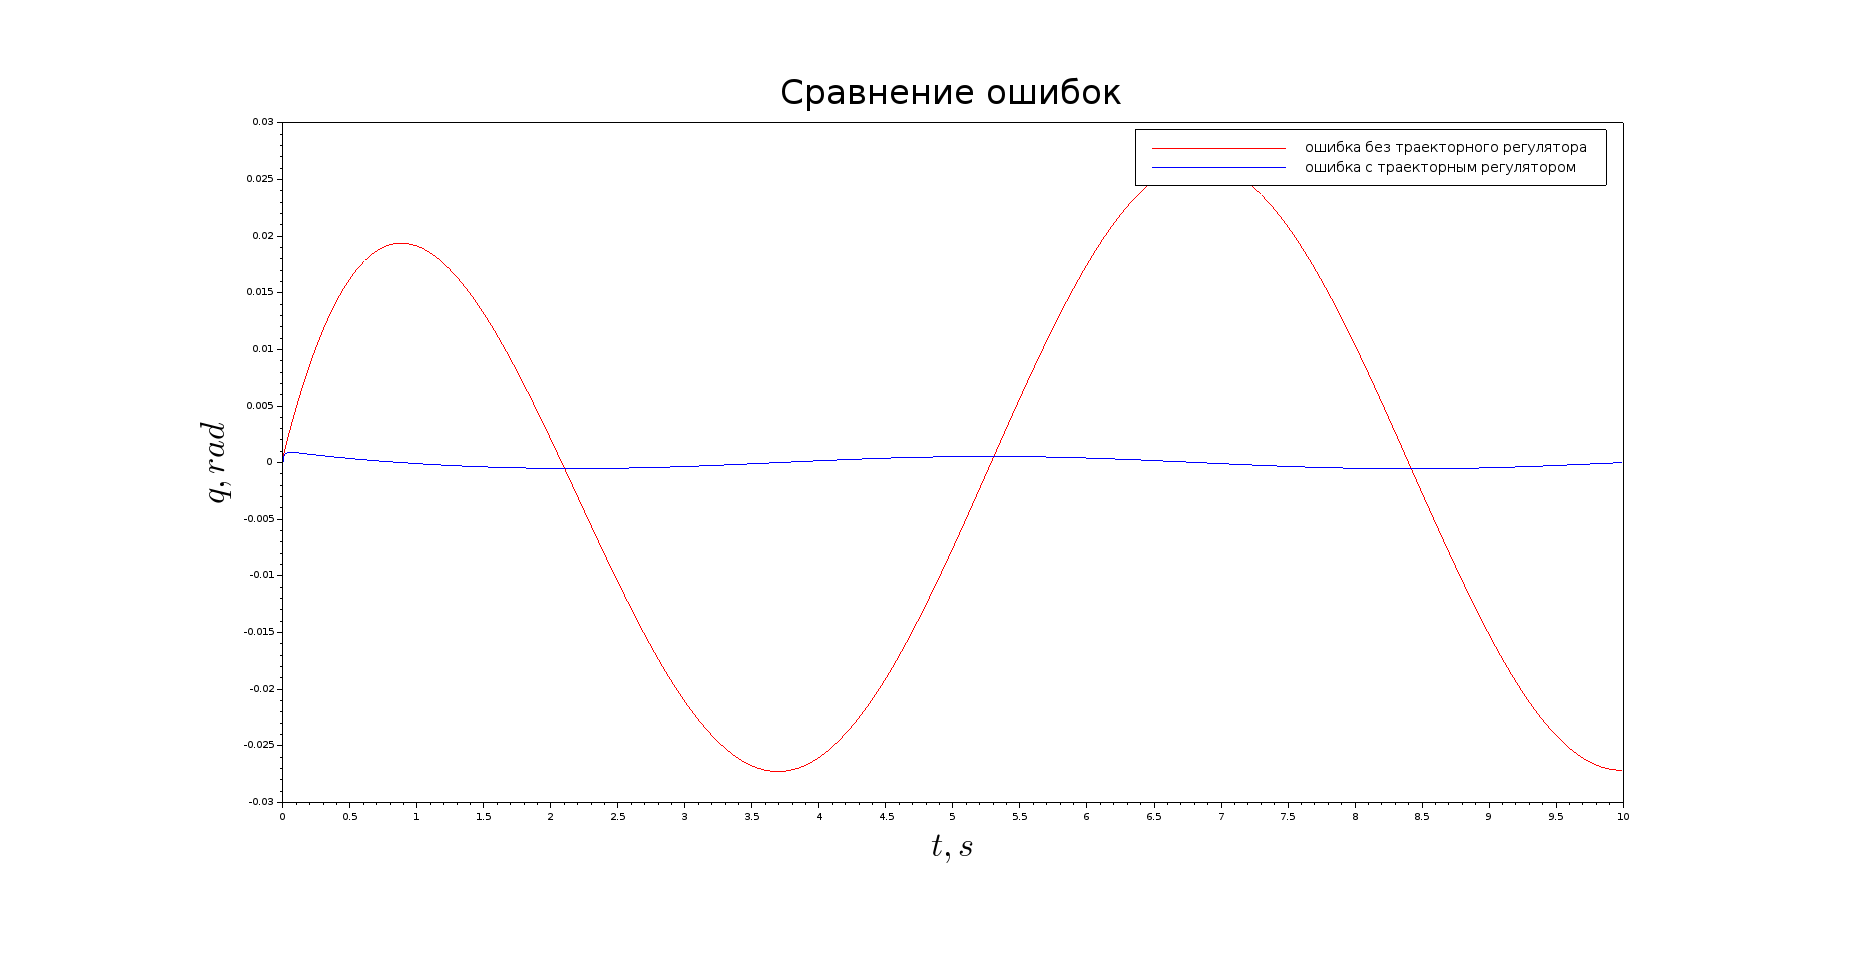
\includegraphics[width=0.8\textwidth]{Lab4/images/Error_comparison.png}\\
    \centering{Рис 4.7 Система моделирования замкнутой системы с ПИД-регулятором}
\end{center}